\section{Cel pracy}
Naszym celem podczas projektowania i implementacji sprzętowo-programowego systemu przetwarzania danych wektorowych było skonstruowanie od podstaw całej ścieżki przetwarzania danych, ze szczególnym uzwględnieniem danych wektorowych. W praktyce inżynierii oprogramowania, czy to w~pracy, czy na uczelni, programista jest zmuszony skupić się na wybranym aspekcie przetwarzania informacji: najczęściej polega to na pisaniu programów na wybraną architekturę, korzystając z ustalonego języka (języków) programowania i~dostarczonych do nich bibliotek. Okazuje się jednak, że przy niektórych szczególnych zastosowaniach, gdzie wymagana jest ogromna szybkość i~przepustowość systemów przetwarzania danych, korzystanie z~ przygotowanych narzędzi może nie być wystarczające. Taka sytuacja ma miejsce na przykład w~zastosowaniach finansowych, w~szczególności przy implementacji algorytmów HFT (High-Frequency Trading), które muszą w~czase rzędu milisekund podejmować decyzje o~sprzedaży bądź kupnie akcji. Okazuje się, że fundusze inwestycyjne zmuszone są inwestować wielkie kwoty nie tylko w~zasoby ludzkie, ale także w~coraz bardziej specjalistyczny i~wydajny sprzęt, by nadążyć za rosnącą szybkością i~objętością transakcji.

Obecnie rynek ten jest zdominowany przez ,,zwykłe'' procesory i~karty graficzne oraz języki programowania takie, jak: {\tt C/C++}, {\tt Python} i~{\tt Java}. Choć ich zaletą jest powszechność, wspomniane rozwiązania mogą okazać się zbyt generyczne, by były naprawdę wydajne. Dla ilustracji przytoczmy prosty przykład: jeśli potrzeby naszego systemu przetwarzania danych sprowadzają się do ustawicznego dodawania wektorów liczb naturalnych, marnotrawstwem zasobów jest opieranie go o~procesor, który potrafi wykonywać również wiele innych operacji, jak na przykład mnożenie i~dzielenie liczb zmiennoprzecinkowych. Zamiast tego warto skonstruować dedykowany procesor, który będzie potrafił tylko dodawać liczby całkowite, ale będzie potrafił dodać ich 2048 w~jednym cyklu zegara. Dodatkowo, system powinien być przyjazny dla programisty, tj. nie można zmuszać programistów do pisania kodu assemblerowego. Idealnym rozwiązaniem jest wysokopoziomowy język programowania, kompilowany i~optymalizowany pod naszą konkretną architekturę.

W niniejszej pracy wysuwamy tezę, że możliwe jest skonstruowanie kompletnego systemu przetwarzania danych opartego na konfigurowalnych układach FPGA i~dedykowanym, wysokopoziomowym języku programowania, który docelowo mógłby stać się alternatywą dla rozwiązań składanych z różnych komponentów. Warto podkreślić, że w~pracy nie stawiano sobie za cel skonstruowanie systemu, który w~obecnej formie mógłby konkurować z~komercyjnymi rozwiązaniami. Celem było pokazanie takiej możliwości przez dostarczenie działającego produktu i~wskazanie kierunku, w~jakim można go rozwijać i~skalować.

\section{Wizja}
System ma umożliwiać użytkownikom przetwarzanie danych w możliwie intuicyjny i~wydajny sposób. Aby to osiągnąć, musi składać się z~trzech głównych części:
\begin{itemize}
  \item języka programowania i kompilatora
  \item modułu odpowiedzialnego za komunikację pomiędzy komputerem PC, na którym działa kompilator i~na którym tworzone są programy oraz procesorem na układzie FPGA
  \item procesora zbudowanego na układzie FPGA
\end{itemize}

\subsection{Język programowania}
Język programowania powinien, w~naszym przekonaniu, z~jednej strony pozwalać programiście na osiągnięcie celu w~jak najłatwiejszy sposób, a~z~drugiej na jak najwcześniejszym etapie (podczas kompilacji) wychwycić błędy w programie tak, by nie tracono czasu na testowanie programu w~oczywisty sposób niepoprawnego. Pociąga to za sobą następujące wytyczne co do języka programowania do zastosowania w~naszym systemie:

\begin{itemize}
  \item statyczne typowanie -- pozwala poinformować w~czasie kompilacji o~typowych błędach jak np. próba dodania skalara do wektora
  \item typy zależne w podstawowym zakresie -- język do obliczeń wektorowych nie powinien pozwolić na, przykładowo, dodanie do siebie dwóch wektorów o~różnej długości
  \item wbudowane w język operacje na wektorach -- aby operować wektorami nie powinno być konieczne odwoływanie się do pamięci czy korzystanie ze specjalnych bibliotek
\end{itemize}

\begin{figure}
  \begin{center}
    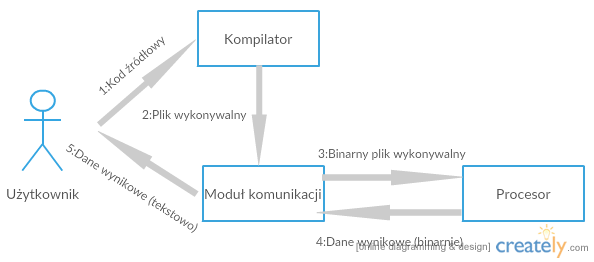
\includegraphics[scale=0.5]{images/SystemOverview.png}
    \caption{Schemat działania systemu. Na diagramie przedstawiono ogólną ideę, wedle której działa system.}
    \label{fig:SystemOverview}
  \end{center}
\end{figure}

\subsection{Procesor}
Procesor powinien być jak najmniej skomplikowany, a~jednocześnie jak najwydajniej wykonywać swoje zadanie. Prostą implikacją tych dwóch wymagań jest architektura ukierunkowana na przetwarzanie wektorów. Operacje na wektorach o~pewnej ustalonej długości powinny odbywać się w~jednym cyklu zegara. Koncepcyjnie jest to zbliżone do AVX w~procesorach firmy Intel. Tam procesory potrafią wykonywać operacje na czterech liczbach zmiennoprzecinkowych w jednym cyklu, jeśli użyjemy specjalnych instrukcji. Nas interesuje dużo ściślejsza integracja wektorowej architektury -- każda instrukcja ma być wektorowa, jako że wektor jest podstawową jednostką danych. Patrząc z~ilościowego punktu widzenia na aplikacje wymagające przetwarzania wektorów, dużo mniej tracimy traktując każdy skalar w~programie jako wektor o~pewnej długości z~jedną niezerową współrzędną, niż indywidualnie przetwarzając każdy element wektora.

Na ogólną wydajność systemu ma wpływ także rozmiar kodu maszynowego generowanego przez kompilator, a~ta jest bezpośrednio zależna od architektury procesora. Panuje zgodna opinia, że najmniejszy rozmiar kodu maszynowego uzyskują procesory działające na zasadzie maszyny stosowej. Oprócz tego dobrze, by każda z instrukcji miała stałą długość (dzięki temu dużo prostsze jest ich dekodowania) oraz by każda z~instrukcji miała niewielką długość. Optymalną długością instrukcji jest jeden bajt -- dzięki temu łatwo jest je przesyłać, a~program zajmuje bardzo niedużo miejsca.

\subsection{Komunikacja}
Moduł komunikacyjny jest oparty na standardzie UART, ale wraz z~rozwojem systemu będzie można zaimplementować szybsze metody komunikacji. UART ma zalety zarówno w postaci stosunkowej łatwości implementacji na układzie FPGA, jak i~łatwości obsługi po stronie komputera PC z~systemem Linux. W przypadku nowych komputerów, które nie posiadają portu RS-232 można zastosować szerokodostępne i~tanie przejściówki USB-UART, które pozwalają nam korzystać z~portu UART z~poziomu programów w~C tak samo, jak z~każdego innego urządzenia wejścia-wyjścia w~systemie.

Potrzebne komponenty to oczywiście moduł UART zaimplementowany na FPGA, jak i~program, który pozwoli na przesyłanie danych pomiędzy komputerem i~koprocesorem. Program powinien prezentować otrzymane od procesora wyniki w~możliwie czytelny sposób tak, by umożliwić ich dalszą analizę.
